% -*- coding: utf-8 -*-
\documentclass[11pt, a4paper]{article}

% ============================================================================
% Encoding & language
% ============================================================================
\usepackage[utf8]{inputenc}
\usepackage[T1]{fontenc}
\usepackage[english]{babel}

% ============================================================================
% Page layout
% ============================================================================
\usepackage[a4paper,
            top=2.5cm, bottom=2.6cm,
            left=2.6cm, right=2.6cm,
            headheight=14pt,
            footskip=1.0cm]{geometry}
\usepackage{parskip}
\setlength{\parskip}{0.55em}
\linespread{1.07}

% ============================================================================
% Fonts
% ============================================================================
\usepackage{libertine}
\renewcommand{\familydefault}{\rmdefault}
\usepackage[T1]{fontenc}
\usepackage{microtype}
\microtypesetup{protrusion=true,expansion=false,tracking=false}

% ============================================================================
% Graphics & figures
% ============================================================================
\usepackage{graphicx}
\usepackage[font=small,labelfont={bf,sf,color=accentdark},
            justification=justified,
            labelsep=period,
            margin=10pt]{caption}
\usepackage{float}
\usepackage{wrapfig}

% ============================================================================
% Color, boxes, rules
% ============================================================================
\usepackage{xcolor}
\definecolor{accentdark}{HTML}{1F3A52}
\definecolor{accent}{HTML}{3D5D75}
\definecolor{accentlight}{HTML}{7F9CB3}
\definecolor{accentwarm}{HTML}{A06030}
\definecolor{accentwarmlight}{HTML}{C09060}
\definecolor{rulegray}{HTML}{C8CDD2}
\definecolor{tldrbg}{HTML}{EAF2F8}
\definecolor{notebg}{HTML}{FFF6E5}
\definecolor{v1bg}{HTML}{EAF2F8}
\definecolor{v2bg}{HTML}{F7EEE2}
\definecolor{quoteleft}{HTML}{A53E2A}
\definecolor{footergray}{HTML}{888888}

\usepackage[most]{tcolorbox}
\tcbset{
    tldr/.style={
        enhanced,
        colback=tldrbg, colframe=accent,
        boxrule=0pt, frame hidden,
        borderline west={2.5pt}{0pt}{accent},
        arc=2pt,
        left=14pt, right=12pt, top=8pt, bottom=8pt,
        fontupper=\small,
    },
    note/.style={
        enhanced,
        colback=notebg, colframe=orange!70!black,
        boxrule=0pt, frame hidden,
        borderline west={2.5pt}{0pt}{orange!70!black},
        arc=2pt,
        left=14pt, right=12pt, top=8pt, bottom=8pt,
        fontupper=\small,
    },
    v1box/.style={
        enhanced,
        colback=v1bg, colframe=accent,
        boxrule=0pt, frame hidden,
        borderline west={3pt}{0pt}{accent},
        arc=2pt,
        left=14pt, right=12pt, top=8pt, bottom=8pt,
    },
    v2box/.style={
        enhanced,
        colback=v2bg, colframe=accentwarm,
        boxrule=0pt, frame hidden,
        borderline west={3pt}{0pt}{accentwarm},
        arc=2pt,
        left=14pt, right=12pt, top=8pt, bottom=8pt,
    },
}

\newcommand{\pullquote}[1]{%
  \begin{center}\vspace{0.3em}%
  \begin{minipage}{0.86\textwidth}%
    \color{quoteleft}\sffamily\itshape\large%
    \rule[-0.4em]{2pt}{1.4em}\hspace{0.6em}#1%
  \end{minipage}\vspace{0.3em}\end{center}}

% ============================================================================
% Section styling
% ============================================================================
\usepackage[explicit]{titlesec}
\titleformat{\section}[block]
  {\normalfont\sffamily\Large\bfseries\color{accentdark}}
  {\thesection}{0.7em}{#1}
  [\vspace{-0.2em}{\color{rulegray}\rule{\linewidth}{0.4pt}}]
\titleformat{\subsection}[block]
  {\normalfont\sffamily\large\color{accent}}
  {\thesubsection}{0.6em}{#1}
\titleformat{\subsubsection}[runin]
  {\normalfont\sffamily\normalsize\bfseries\color{accent}}
  {}{0em}{#1\enspace---\enspace}
\titlespacing*{\section}{0pt}{1.6em}{0.6em}
\titlespacing*{\subsection}{0pt}{1.0em}{0.3em}
\titlespacing*{\subsubsection}{0pt}{0.6em}{0.3em}

% ============================================================================
% Tables
% ============================================================================
\usepackage{booktabs}
\usepackage{array}
\usepackage{tabularx}
\newcolumntype{L}{>{\raggedright\arraybackslash}X}
\renewcommand{\arraystretch}{1.25}

% ============================================================================
% Headers/footers
% ============================================================================
\usepackage{fancyhdr}
\pagestyle{fancy}
\fancyhf{}
\renewcommand{\headrulewidth}{0pt}
\renewcommand{\footrulewidth}{0pt}
\fancyhead[L]{\small\sffamily\color{accentlight}From Permafrost to Music}
\fancyhead[R]{\small\sffamily\color{accentlight}Methods overview}
\fancyfoot[C]{\small\sffamily\color{footergray}\thepage}

\fancypagestyle{cover}{%
  \fancyhf{}%
  \renewcommand{\headrulewidth}{0pt}%
  \renewcommand{\footrulewidth}{0pt}%
}

% ============================================================================
% TOC styling
% ============================================================================
\usepackage[titles]{tocloft}
\renewcommand{\cfttoctitlefont}{\Large\sffamily\bfseries\color{accentdark}}
\renewcommand{\cftsecfont}{\normalfont\sffamily}
\renewcommand{\cftsecpagefont}{\normalfont\sffamily\color{accent}}
\renewcommand{\cftsubsecfont}{\normalfont\sffamily\small\color{accent}}
\renewcommand{\cftsubsecpagefont}{\normalfont\sffamily\small\color{accent}}
\setlength{\cftbeforesecskip}{0.6em}
\renewcommand{\cftdotsep}{2}

% ============================================================================
% Hyperref last
% ============================================================================
\usepackage[
  colorlinks=true,
  linkcolor=accent,
  urlcolor=accent,
  citecolor=accent,
  pdftitle={From Permafrost to Music --- Methods overview},
  pdfauthor={soil-audio pipeline},
  pdfsubject={Sonification methodology --- two delivered versions},
]{hyperref}

\graphicspath{{outputs/report_figs/}}

% ============================================================================
% Document
% ============================================================================
\begin{document}

% ---------- COVER PAGE ----------
\thispagestyle{cover}
\begin{flushleft}
  \vspace*{2em}
  {\sffamily\color{accentlight}\large soil-audio \,/\, methods overview}\par
  \vspace{1.5em}
  {\color{rulegray}\rule{0.55\linewidth}{0.5pt}}\par
  \vspace{1.0em}
  {\sffamily\color{accentdark}\fontsize{32pt}{36pt}\selectfont\bfseries From Permafrost\\to Music}\par
  \vspace{0.8em}
  {\sffamily\color{accent}\Large Two delivered sonifications of Tasiujaq soil temperature data}\par
  \vspace{2.5em}
\end{flushleft}

\begin{figure}[H]
  \centering
  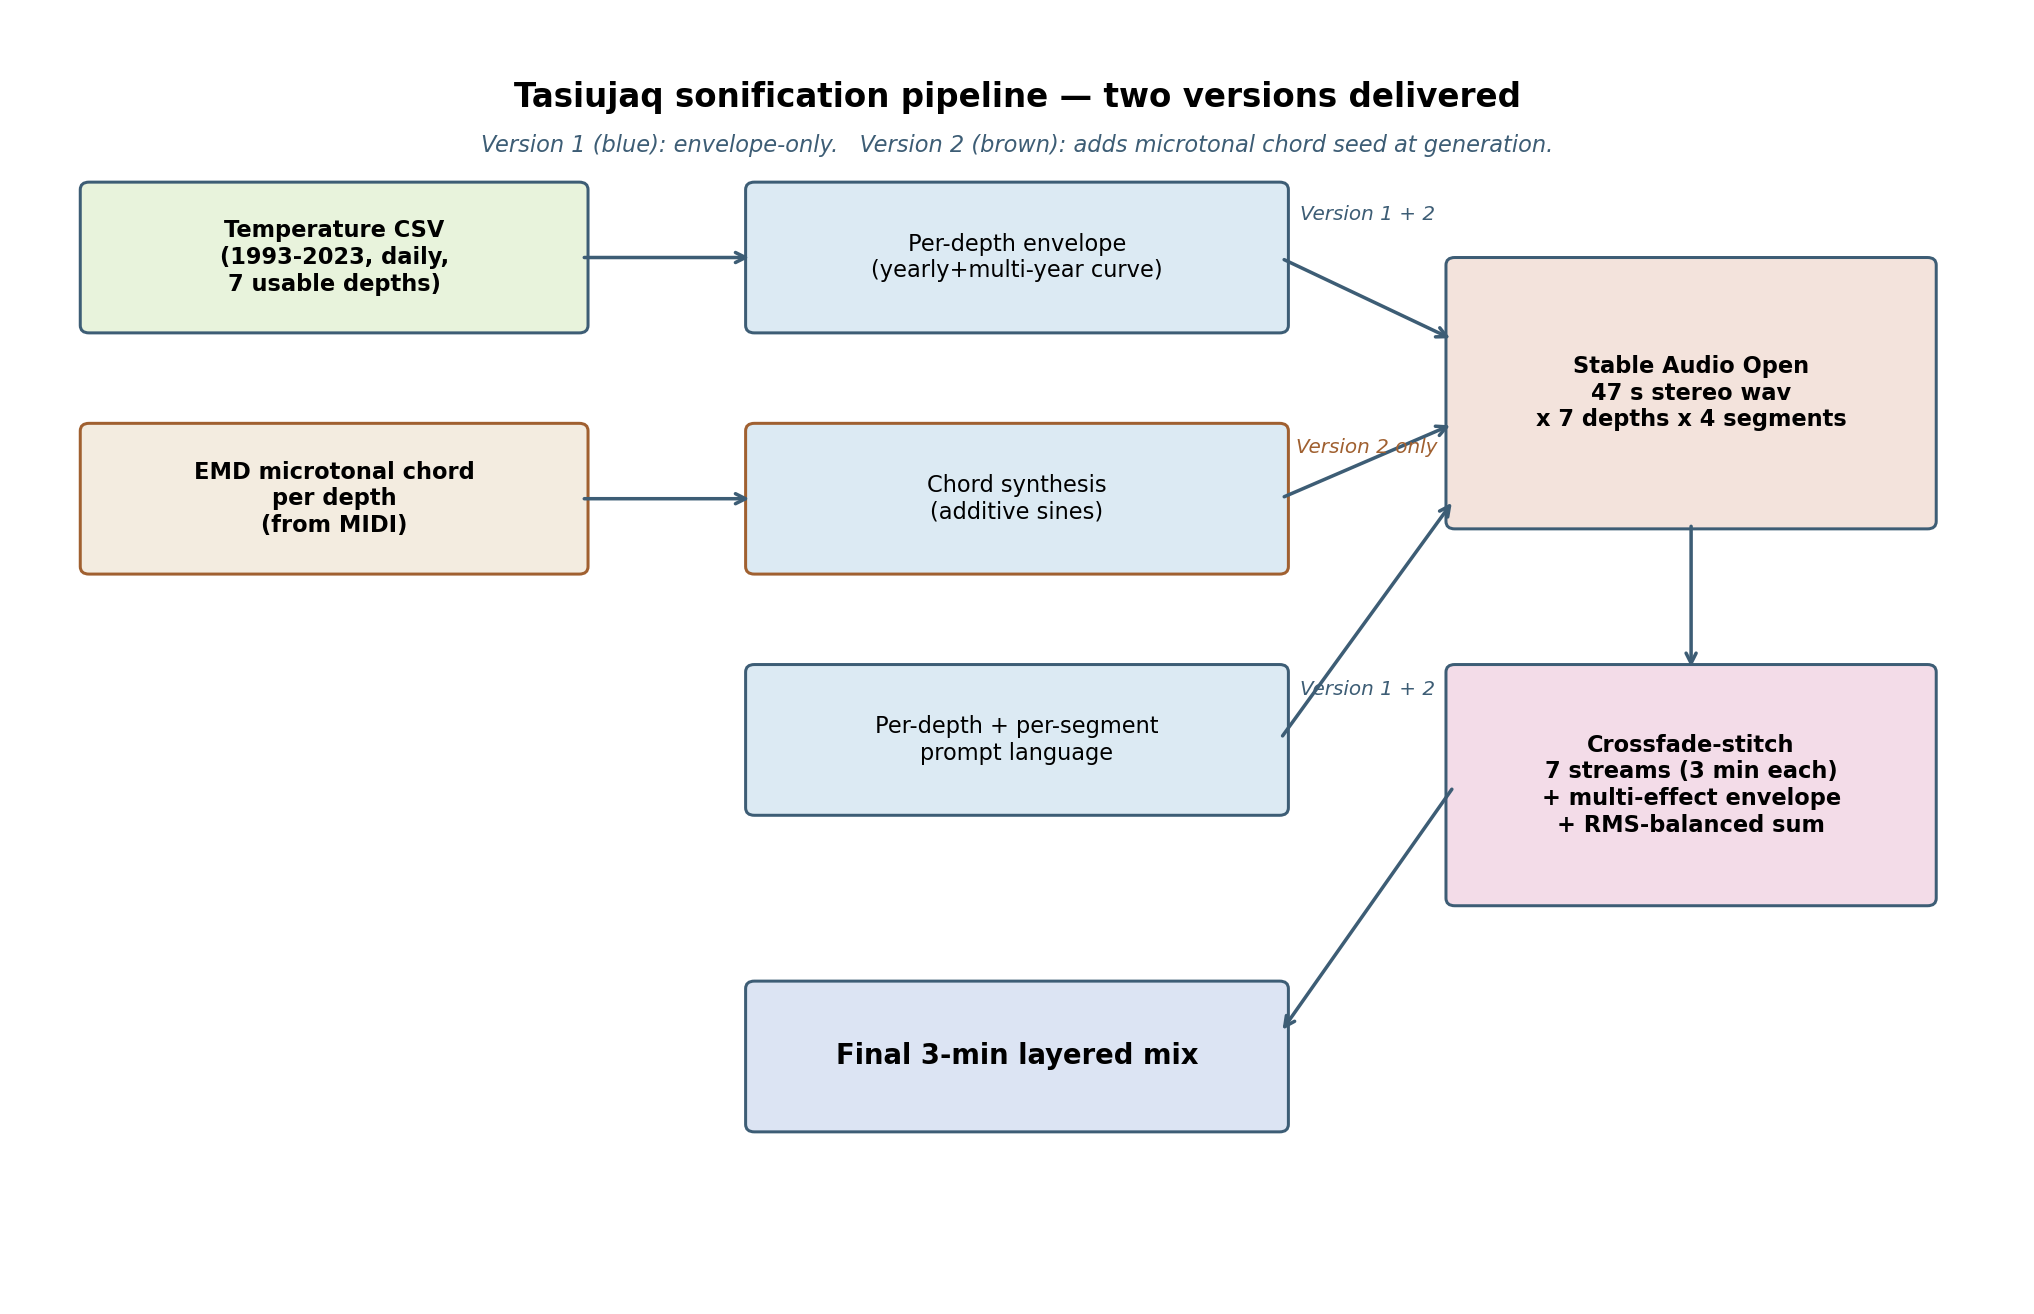
\includegraphics[width=0.96\linewidth]{01_pipeline.png}
\end{figure}

\vspace{1.0em}
\begin{tcolorbox}[tldr]
\noindent\textbf{Summary.}\enspace
We turn 27 years of daily soil-temperature data from Tasiujaq (1993--2023)
into two complementary 3-minute orchestral pieces. Both pieces share the same
seven musical voices (one per soil depth between 200~cm and 1100~cm), the same
prompt-driven instrument design, and the same envelope-shaping stage.
They differ in \emph{how the data couples to the generated audio}:

\medskip
\noindent\textbf{Version 1 --- Envelope-modulated sonification.}\enspace
The soil signal shapes each voice via a per-depth audio effect: loudness,
brightness, stereo width, tremolo, or bass cut, chosen so each voice
expresses the data in a different sensory dimension.

\medskip
\noindent\textbf{Version 2 --- Microtonal-anchored sonification.}\enspace
In addition to the envelope shaping, the microtonal harmonic content of each
depth (extracted by EMD) is fed directly into the AI model's diffusion
process as an initial seed. The model's generated pitches are then biased
toward the depth's actual microtonal chord. The data couples to the music
both in time (envelope) and in spectrum (chord).
\end{tcolorbox}

\vfill
\begin{flushleft}
  {\sffamily\footnotesize\color{footergray}
  Methods overview --- two-version edition.\\
  Prepared from the project's data and code.}
\end{flushleft}

\clearpage

% ---------- TABLE OF CONTENTS ----------
\thispagestyle{cover}
\vspace*{1em}
\renewcommand{\contentsname}{Contents}
\tableofcontents
\vfill
\clearpage

\setcounter{page}{1}

% ============================================================================
\section{The source data}
% ============================================================================

The input is a CSV file of soil temperatures measured at fourteen depths
between $0$~cm (surface) and $1100$~cm (eleven metres below ground) at
Tasiujaq, Nunavik. Measurements are daily and span 26.7 years (9{,}748 days,
August 1993 through 2023). Seven of the fourteen depths have sufficiently
continuous coverage to be usable in the piece: $200$, $300$, $400$, $500$,
$700$, $900$ and $1100$~cm.

The depths tell radically different physical stories. Near the surface, the
soil follows the seasons aggressively --- summer warming pushes temperatures
up past $+20\,^{\circ}\mathrm{C}$, while winter air drops them below
$-30\,^{\circ}\mathrm{C}$. Heat diffuses slowly into the earth, so every
additional metre of depth smooths and delays this signal. By $11$~m deep,
temperatures hover narrowly between $-5$ and $-4\,^{\circ}\mathrm{C}$ all
year round --- that is the permafrost, almost motionless across the full
27-year record.

A complementary input is also available: an \emph{Empirical Mode
Decomposition} (EMD) of the same soil signal, exported as a microtonal MIDI
file. For each usable depth, the EMD analysis produces 8--11 frequencies
spread across roughly eight octaves --- a per-depth ``chord'' that
characterises the depth's internal harmonic structure. The lowest of these
frequencies is always around 28--32~Hz; this shared sub-bass anchor reflects
the multi-decade temperature trend that every depth ultimately responds to.

\pullquote{Volatile soil $\to$ expressive voice. Stable soil $\to$ drone.}

% ============================================================================
\section{From depth to voice}
% ============================================================================

Each of the seven usable depths is assigned its own musical voice ---
an instrument or vocal layer described in prose and fed to the AI model as a
text prompt. The voices are deliberately spread across distinct frequency
bands and roles so they layer transparently rather than crowd the same
range.

\begin{figure}[H]
  \centering
  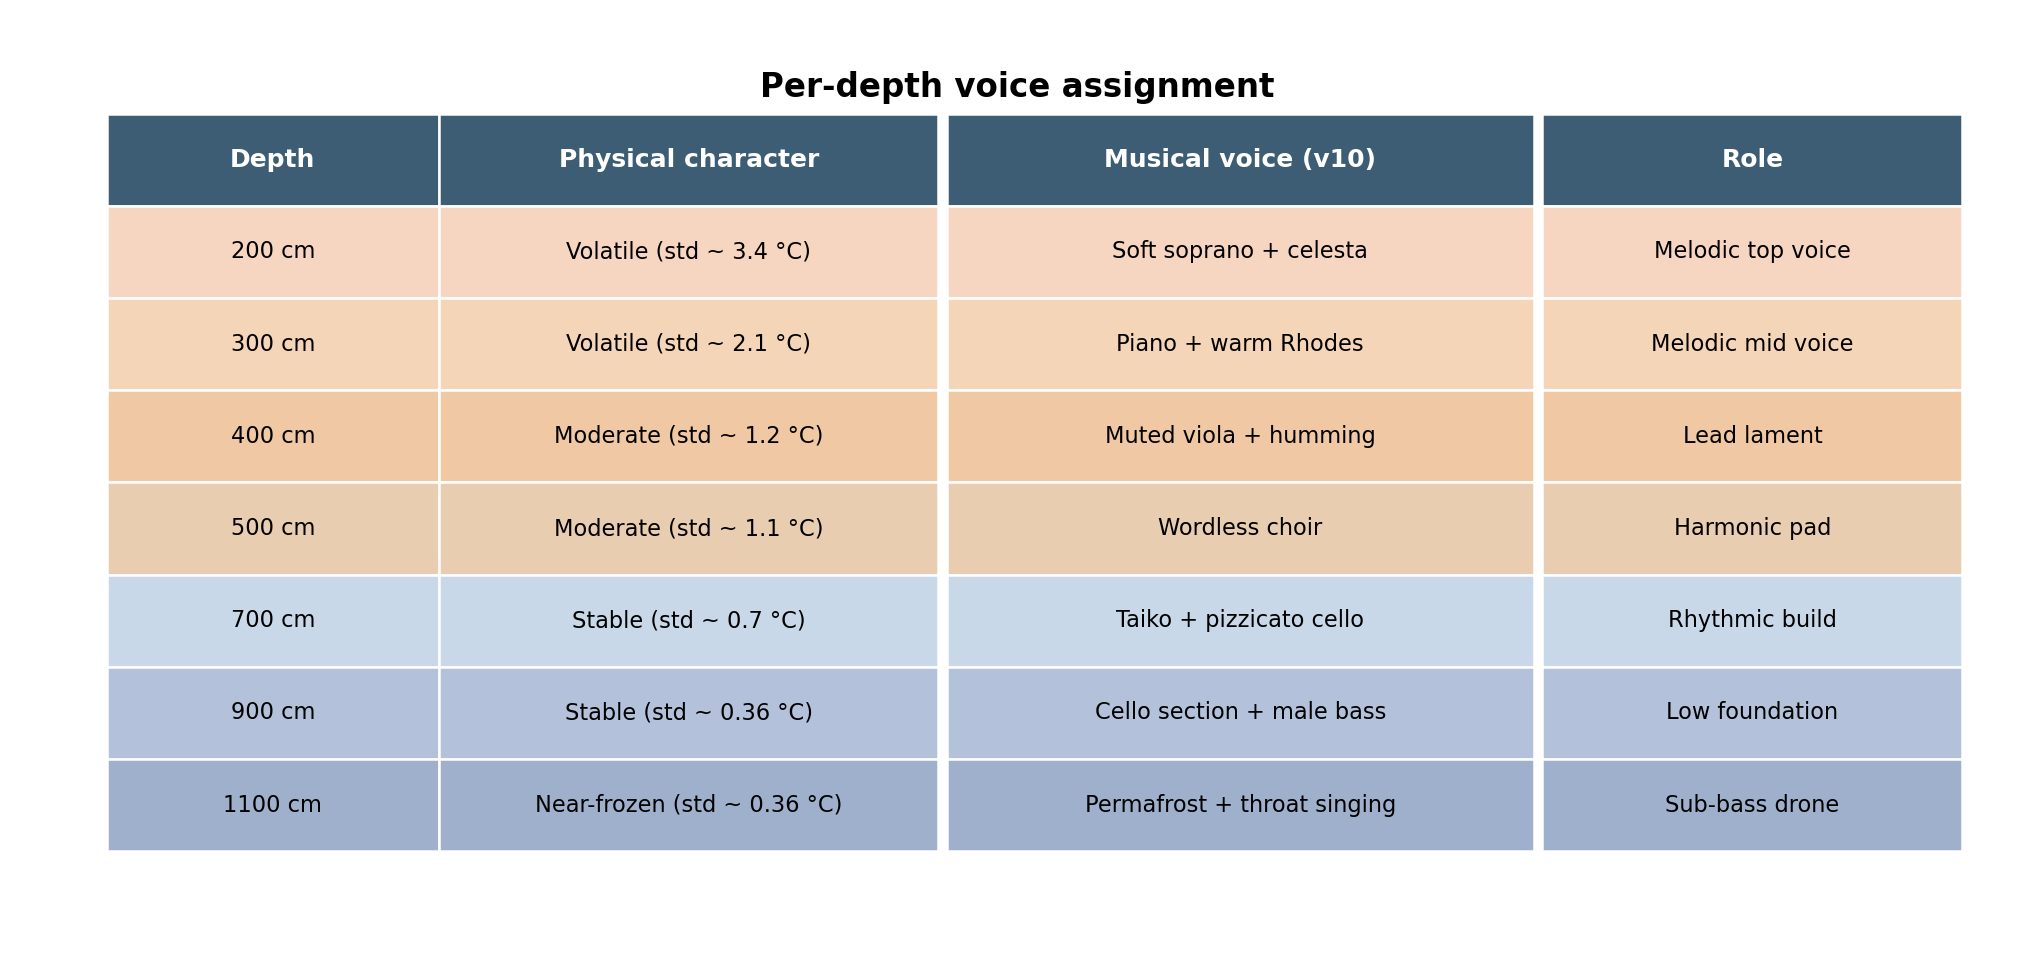
\includegraphics[width=\linewidth]{02_depth_voices.png}
  \caption{Per-depth voice assignment, shared by both versions. Warm tones at
  the top are the most expressive and melodic; cool tones at the bottom hold
  the drone foundation. Surface stems contain the more delicate, transient
  elements (voice, celesta); deep stems are sustained and in the low
  register.}
  \label{fig:depthvoices}
\end{figure}

% ============================================================================
\section{Mapping 27 years onto 3 minutes}
% ============================================================================

The AI audio model's hard architectural maximum output is 47~seconds. To
produce a 3-minute piece we split the audio into four 47-second segments
crossfaded together (3-second equal-power crossfades, giving
$4 \times 47 - 3 \times 3 \approx 179$~s). We use this constraint to our
narrative advantage: each segment is fed a different $\sim 6.7$-year slice of
the soil record, so the multi-decade warming trend is embedded in the
music's progression.

\begin{figure}[H]
  \centering
  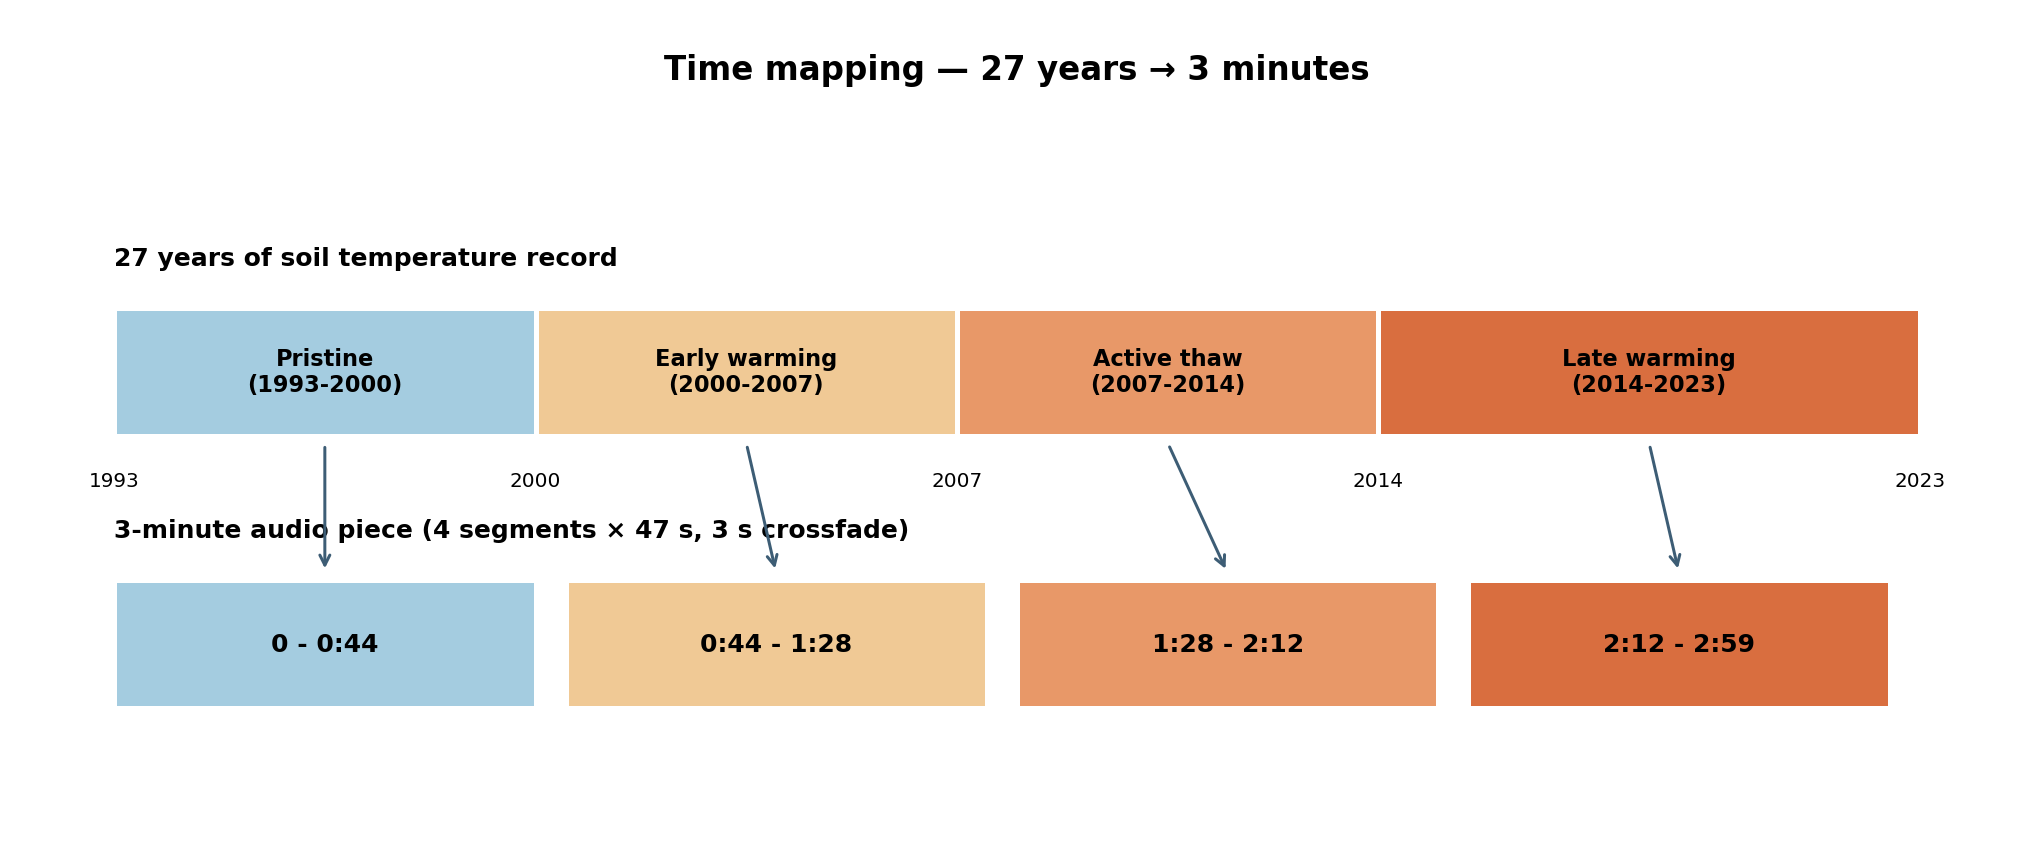
\includegraphics[width=\linewidth]{03_segments_timeline.png}
  \caption{Time mapping. The 27-year record is divided into four windows of
  about 6.7 years each. Each window drives one $\sim47$-second audio segment;
  all four are crossfaded together into the final $\sim3$-minute piece.
  Prompt descriptors evolve in parallel --- ``pristine'' at the start,
  ``active thaw'' in the middle, ``late warming'' at the end.}
  \label{fig:timeline}
\end{figure}

\begin{tcolorbox}[note,title={\textbf{Each segment carries $\sim 6.7$ years, not 1 year}}]
Because each 47-second segment is driven by $\sim 6.7$ years of daily
temperature data, every segment contains roughly seven seasonal cycles of
the soil signal. The envelope therefore oscillates at both a slow
multi-year scale (the climate trend) and a faster yearly scale (the
seasons) within each 47-second window.
\end{tcolorbox}

% ============================================================================
\section{The shared mechanism: envelope extraction}
\label{sec:envelope}
% ============================================================================

Both versions share the same first stage: for each depth and each segment,
the actual temperature curve is converted into an \emph{envelope} ---
a single curve in $[0, 1]$ that follows the soil signal in time. That
envelope is what sculpts the AI-generated audio in the second stage.

\begin{figure}[H]
  \centering
  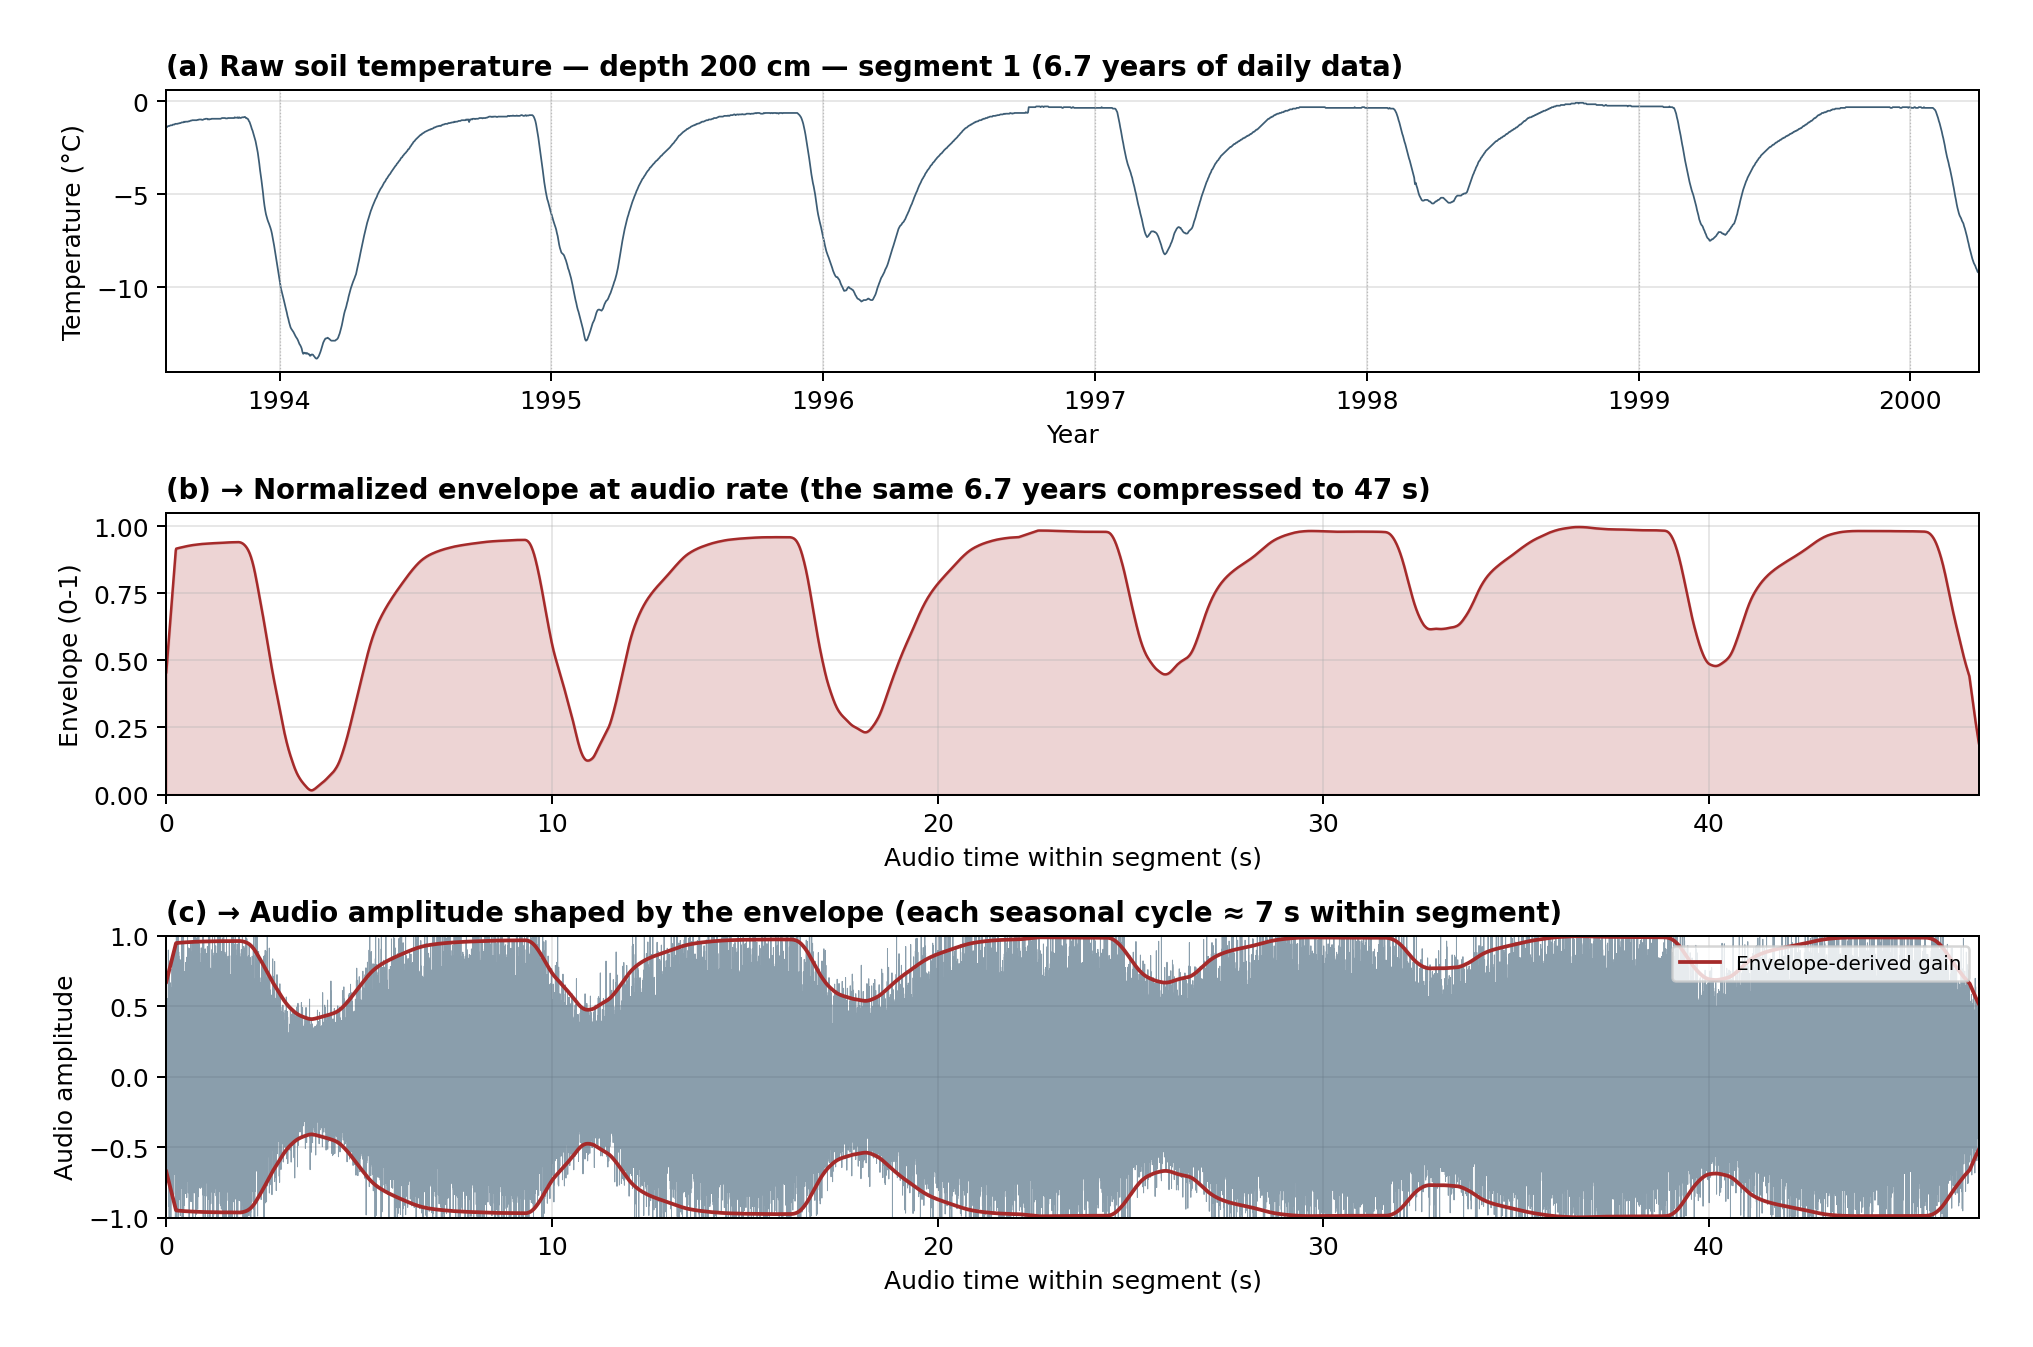
\includegraphics[width=\linewidth]{04_envelope_concept.png}
  \caption{The three-stage transformation, depth 200~cm, first segment
  (1993--2000). \textbf{(a)} About 6.7 years of daily temperature data ---
  seven seasonal cycles are clearly visible. Vertical dotted lines mark
  January~1; troughs land near January (winter), peaks land mid-year
  (summer). \textbf{(b)} The same shape is normalised to $[0,1]$, smoothed,
  and resampled onto the audio time grid; each year occupies $\sim 7$
  seconds within the 47-second segment. \textbf{(c)} The envelope sculpts a
  synthesised waveform: loudness and other effects breathe with the
  seasons.}
  \label{fig:envelope}
\end{figure}

The audio that the envelope shapes is produced by \emph{Stable Audio
Open~1.0}, an open-weights text-to-audio model run locally on a single GPU.
For each combination of depth $\times$ segment we write a tailored prompt
describing the voice's instrument, register, and segment-specific mood.
With seven depths and four segments per depth, the model is invoked
$28$ times per piece. Generation is deterministic given a fixed random
seed.

\clearpage

% ============================================================================
\section{Version 1 --- Envelope-modulated sonification}
\label{sec:v1}
% ============================================================================

\begin{tcolorbox}[v1box]
\textbf{Version 1 in one line.}\enspace
The AI generates each voice from a text prompt. The depth's temperature
envelope then drives \emph{one} signature audio effect on that voice ---
chosen so each voice expresses the data in a different sensory dimension.
\end{tcolorbox}

\subsection{Per-depth effect routing}

The amplitude envelope is always applied (loudness rises and falls with
warmth). On top of that, each depth gets one additional, voice-appropriate
effect. The routing is intentional: bright, melodic voices receive an
effect that varies their brightness or spatial presence; foundational drones
receive a low-frequency effect that lets the listener hear the bass
``thaw'' as the soil warms; rhythmic voices keep amplitude only, so the
listener can still feel the rhythm clearly.

\begin{tabularx}{\linewidth}{@{}>{\sffamily}l L L@{}}
  \toprule
  \textbf{Depth} & \textbf{Voice} & \textbf{Envelope-driven effect (cold $\to$ warm)} \\
  \midrule
  200~cm  & Soprano + celesta        & \textbf{Stereo width.} Intimate $\leftrightarrow$ wide. \\
  300~cm  & Piano + warm Rhodes      & \textbf{Low-pass cutoff.} Muffled $\leftrightarrow$ bright. \\
  400~cm  & Muted viola + humming    & \textbf{Tremolo depth.} Steady $\leftrightarrow$ trembling. \\
  500~cm  & Wordless choir           & \textbf{Stereo width.} Narrow $\leftrightarrow$ wide. \\
  700~cm  & Taiko + male bass voice  & None (amplitude only --- preserves rhythmic clarity). \\
  900~cm  & Cellos + male bass voice & \textbf{High-pass cutoff.} Bass cut $\leftrightarrow$ full bass. \\
  1100~cm & Permafrost + throat singing & None (amplitude only --- subtle drone). \\
  \bottomrule
\end{tabularx}

\subsection{Implementation}

All envelope-driven filters are implemented as a sample-wise crossfade
between a pre-computed fully-filtered version of the signal and the dry
signal --- this avoids the audible transients that block-wise IIR filtering
produces when the cutoff sweeps quickly. Tremolo is implemented as a
low-rate LFO whose \emph{depth} is modulated by the envelope (steady when
cold, trembling when warm). Stereo width modulates the mid/side ratio.

\pullquote{The same temperature curve sculpts seven voices, each in its own way.}

% ============================================================================
\section{Version 2 --- Microtonal-anchored sonification}
\label{sec:v2}
% ============================================================================

\begin{tcolorbox}[v2box]
\textbf{Version 2 in one line.}\enspace
Same envelope effects as Version 1, plus: the depth's EMD-derived microtonal
chord is fed to the AI model as an \emph{initial seed} of the diffusion
process. The model's generated pitches are biased toward that chord ---
the soil data couples to the music both in time \emph{and} in spectrum.
\end{tcolorbox}

\subsection{The chord seed}

For each depth, the partials extracted from the microtonal MIDI are
synthesised as an additive-sine 47-second stereo clip. Partials above
2~kHz are dropped (they would inject strident high content) and the
remaining partials are weighted so that the lowest frequencies dominate.

\begin{figure}[H]
  \centering
  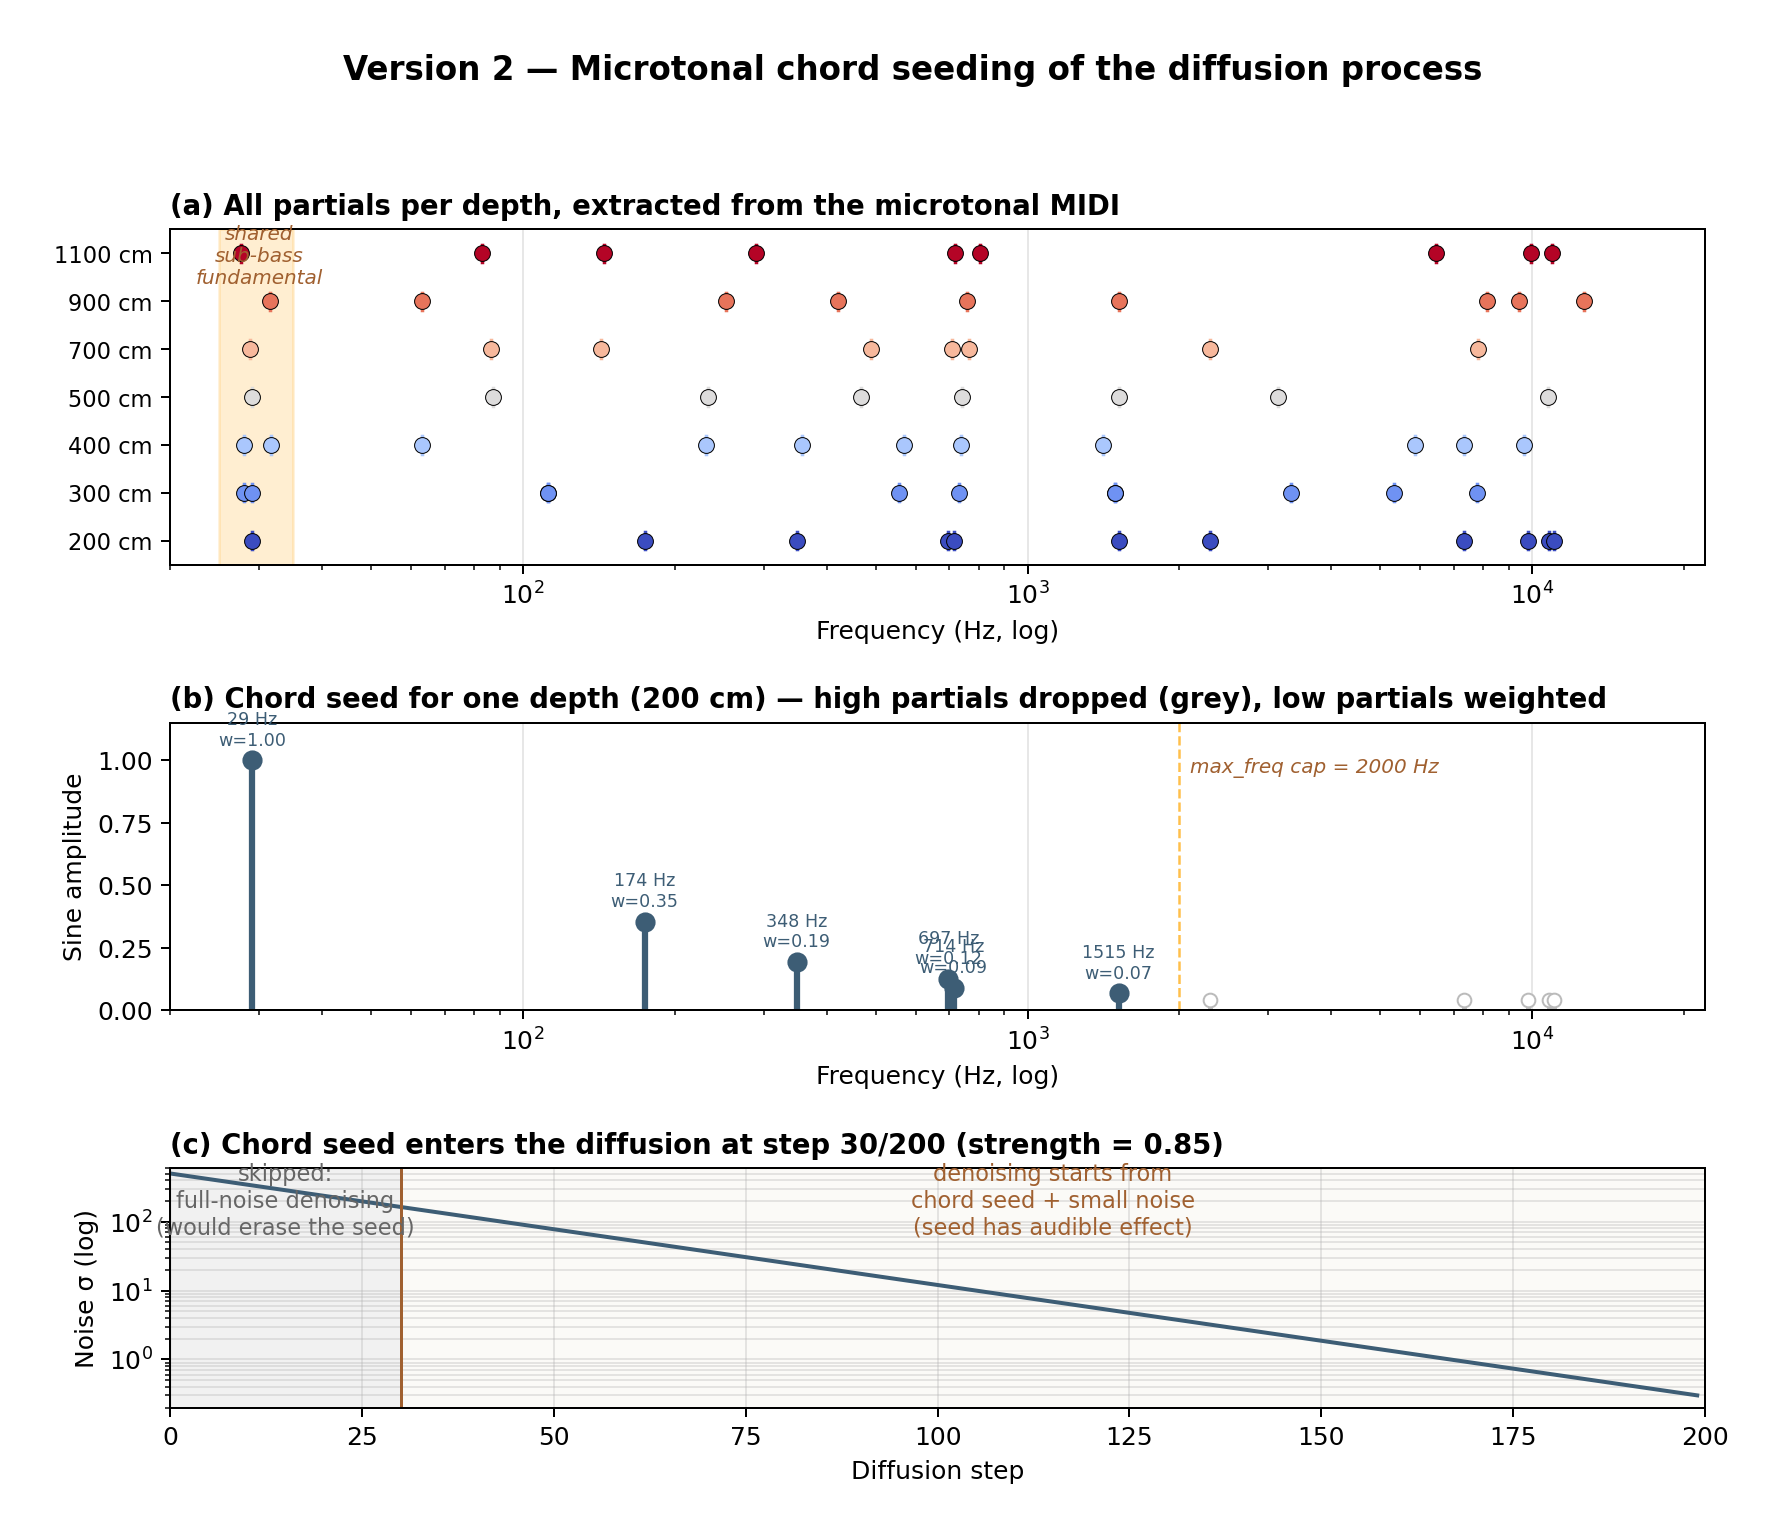
\includegraphics[width=\linewidth]{06_chord_seed.png}
  \caption{Construction and integration of the Version 2 chord seed.
  \textbf{(a)}~The full partial set per depth, as extracted from the
  microtonal MIDI. The orange band marks the shared sub-bass fundamental
  near $30$~Hz that links all seven depths into one harmonic family.
  \textbf{(b)}~For one depth (200~cm), the partials kept (blue) and
  dropped (grey) after the high-frequency cap, with the per-partial
  amplitude weights used in additive synthesis.
  \textbf{(c)}~Where the chord seed enters the diffusion process: instead
  of starting denoising from the full-noise step (which would erase the
  seed), we skip the first 85\% of the noise schedule and begin denoising
  from a much smaller starting noise. The seed therefore has an audible
  effect on the final spectrum.}
  \label{fig:chordseed}
\end{figure}

\subsection{How the seed enters the diffusion}

In a standard text-to-audio generation, the model starts from pure noise
and gradually denoises into audio that matches the text prompt. When an
initial audio is provided, the standard pipeline still adds full-magnitude
noise on top of it before the first denoising step, which effectively
washes out any influence of the seed. Version 2 uses an
\emph{img2img-style} variant: the noise added to the encoded chord seed is
scaled to a much smaller level, and the denoising loop is shortened to
start from that point onwards. The model now operates on a latent that is
genuinely a noisy version of the chord, and its denoising path is pulled
toward the chord's spectrum.

A single parameter, the \emph{strength}, controls the trade-off: at
$\textit{strength}=1.0$ the seed is ignored (stock behaviour); at lower
values the model is increasingly committed to the seed's spectrum. In
practice we use $\textit{strength} \approx 0.85$ --- the seed shapes the
spectrum without overpowering the model's creative content.

\subsection{What is shared with Version 1}

The per-depth multi-effect routing table from Section~\ref{sec:v1} is
applied unchanged to Version 2's audio. The chord seed shapes \emph{what
notes the model plays}; the envelope effects then shape \emph{how those
notes are heard over time}. The data thus couples to the music in two
orthogonal dimensions.

\clearpage

% ============================================================================
\section{Assembly: stitching and mixing}
% ============================================================================

Each depth's four segments are crossfaded together (3-second equal-power
crossfades) into a single $\sim 3$-minute stream. The seven streams are
then loudness-balanced and summed into the final mix. The same assembly
stage is used for both versions.

\begin{figure}[H]
  \centering
  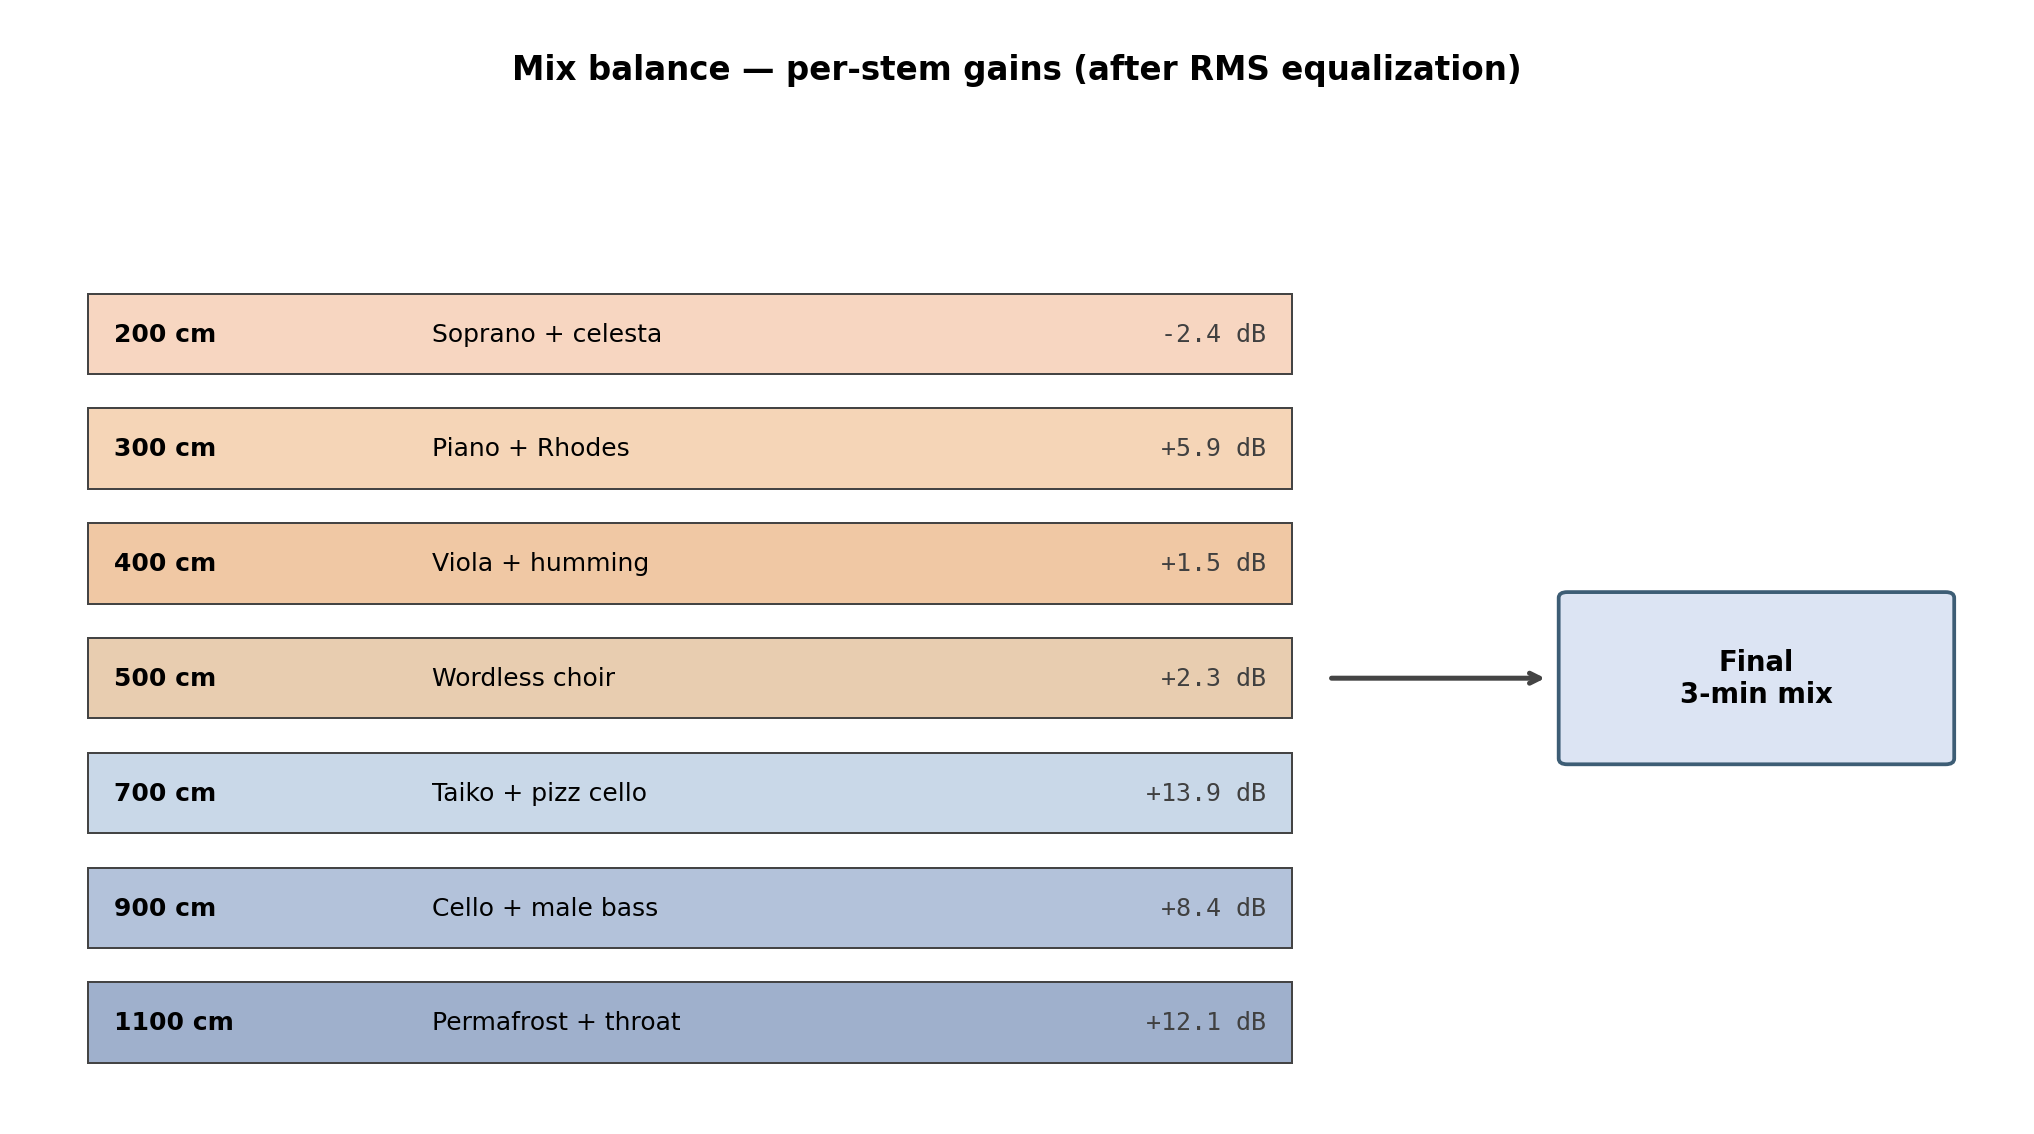
\includegraphics[width=\linewidth]{05_mix_stack.png}
  \caption{Mix balance. The seven streams and their final gains in the
  delivered mixes. Sparse, transient stems (such as the taiko drums or
  the permafrost sub-bass) receive larger boosts (up to $+12$~dB) to
  perceptually match the dense, sustained stems (such as the choir). The
  dB numbers next to each stem are the total gain applied via a two-step
  process: RMS equalisation (lifts sparse stems to the common loudness
  target) and a small manual fader adjustment per stem.}
  \label{fig:mix}
\end{figure}

% ============================================================================
\section{Roadmap}
% ============================================================================

\subsubsection{Multi-IMF envelopes}
Each depth's temperature signal can itself be decomposed by EMD into a
short list of frequency components (daily, seasonal, multi-year). Routing
\emph{different} IMFs to different effects on the same voice ---
e.g.\ the multi-year trend driving filter cutoff while the seasonal cycle
drives loudness --- would give three data-driven control streams per
depth instead of one. No additional AI compute needed; only an iteration
on the envelope-shaping stage.

\subsubsection{Path~B --- envelope-conditioned generation}
A more ambitious extension is to make the AI itself plan its dynamics so
that the generated audio's natural loudness curve already matches the soil
envelope, rather than having the envelope applied afterwards. This is
achievable via inference-time optimisation of the initial noise latent
(DITTO-style methods). Compute cost is roughly $10\times$ the current
pipeline.

\subsubsection{Path~B$^{\!+}$ --- multi-target conditioning}
The same inference-time optimisation can target both the envelope
\emph{and} the spectrum simultaneously, using the chord seed as a spectral
target and the temperature curve as an envelope target. This would unify
Versions 1 and 2 into a single conditioning pass rather than a two-stage
pipeline.

\vspace{2em}
\begin{flushleft}
{\sffamily\small\color{footergray}%
\textbf{Provenance.}\enspace%
Source data: Tasiujaq permafrost monitoring (1993--2023).
Audio model: Stable Audio Open 1.0 (Stability AI).
Pipeline implementation: this project, Python 3.12 with
\texttt{diffusers}, \texttt{scipy}, \texttt{matplotlib}.
Report typeset with \LaTeX{} (Tectonic), Linux Libertine type.}
\end{flushleft}

\end{document}
